%%%%%%%%%%%%%%%%%%%%%%%%%%%%%%%%%%%%%%%%%%%%%%%%%%%%%%%%%%%%%%%%%%%%%%%%
%     LaTeX source code to approximate a Draft NIST Technical report
%	  Instructions for authors: tinyurl.com/techpubsnist 
%	DOI watermark will be added on final PDF
% 	Developed by K. Miller, kmm5@nist.gov 
%	Last updated: 22-March-2019
%%%%%%%%%%%%%%%%%%%%%%%%%%%%%%%%%%%%%%%%%%%%%%%%%%%%%%%%%%%%%%%%%%%

%%%%%%%%%%%%%%%%%%%%%%
% Template further altered by Armen Amirkhanian
% for use with UA lab courses in an effort to 
% have a standardized format for lab documents
% Last update 9-April-2020
%
% TODO:
% --Get the appendices to dynamically link, tocloft causes problems
%%%%%%%%%%%%%%%%%%%%%%

\documentclass[12pt]{article}
\usepackage{amsmath}
\usepackage{amsfonts}   % if you want the fonts
\usepackage{amssymb}    % if you want extra symbols
\usepackage{graphicx}   % need for figures
\usepackage{xcolor}
\usepackage{bm}
\usepackage{secdot}		
\usepackage{mathptmx}
\usepackage{float}
\usepackage[utf8]{inputenc}
\usepackage{textcomp}
\usepackage[hang,flushmargin,bottom]{footmisc} % footnote format
\usepackage{xspace}
%\usepackage{lineno}
\usepackage{ragged2e}
\usepackage{parskip}

\usepackage{tikz}
\usetikzlibrary{shapes.geometric, arrows}
\tikzstyle{startstop} = [rectangle, rounded corners, minimum width=2cm, minimum height=1cm,text centered, draw=black, fill=red!20]
\tikzstyle{arrow} = [thick,->,>=stealth]

\usepackage{titlesec}
\titleformat{\section}{\normalsize\bfseries}{\thesection.}{1em}{}	% required for heading numbering style
\titleformat*{\subsection}{\normalsize\bfseries}

\usepackage{tocloft}	% change typeset, titles, and format list of appendices/figures/tables
\renewcommand{\cftdot}{}	
\renewcommand{\contentsname}{Table of Contents}
\renewcommand{\cftpartleader}{\cftdotfill{\cftdotsep}} % for parts
\renewcommand{\cftsecleader}{\cftdotfill{\cftdotsep}}
\renewcommand\cftbeforesecskip{\setlength{4pt}{}}
\addtolength{\cftfignumwidth}{1em}
\renewcommand{\cftfigpresnum}{\figurename\ }
\addtolength{\cfttabnumwidth}{1em}
\renewcommand{\cfttabpresnum}{\tablename\ }
\setlength{\cfttabindent}{0in}    %% adjust as you like
\setlength{\cftfigindent}{0in} 

\usepackage{enumitem}         % to control spacing between bullets/numbered lists

\usepackage[numbers,sort&compress]{natbib} % format bibliography 
\renewcommand{\bibsection}{}
\setlength{\bibsep}{0.0pt}

\usepackage[hidelinks]{hyperref}
\hypersetup{
	colorlinks = true,
urlcolor ={blue},
citecolor = {.},
linkcolor = {.},
anchorcolor = {.},
filecolor = {.},
menucolor = {.},
runcolor = {.}
pdftitle={},
pdfsubject={},
pdfauthor={},
pdfkeywords={}
}
\urlstyle{same}

\usepackage{epstopdf} % converting EPS figure files to PDF

\usepackage{fancyhdr, lastpage}	% formatting document, calculating number of pages, formatting headers
\setlength{\topmargin}{-0.5in}
\setlength{\headheight}{39pt}
\setlength{\oddsidemargin}{0.25in}
\setlength{\evensidemargin}{0.25in}
\setlength{\textwidth}{6.0in}
\setlength{\textheight}{8.5in}

\usepackage{caption} % required for Figure labels
\captionsetup{font=small,labelfont=bf,figurename=Fig.,labelsep=period,justification=raggedright} 

%%%%%%%%%%% !!!!!REQUIRED - FILL OUT METADATA HERE !!!!!!!! %%%%%%%%%%%%%%
%%%%%%%%%%%%%%%%%%%%%%%%%%%%%%%%%%%%%%%%%%%%%%%%%%%%%%%%%%%%%%%%%%%%%%%%%%
\newcommand{\CourseNum}{CE262}
\newcommand{\CourseName}{Civil Engineering Materials}
\newcommand{\LabTitle}{Sieve Analysis}
\newcommand{\LastUpdate}{Fall 2020}

%%%%%%%%%%%%%%%%%%%%%%%%%%%%%%%%%%%%%%%%%%%%%%%%%%%%%%%%%%%%%%%%%%%%
%   	BEGIN DOCUMENT 
%%%%%%%%%%%%%%%%%%%%%%%%%%%%%%%%%%%%%%%%%%%%%%%%%%%%%%%%%%%%%%%%%%%%
\begin{document}
	\urlstyle{rm} % Format style of \url   
%\linenumbers
\begin{titlepage}
\begin{flushright}
\LARGE{\textbf{\CourseNum{} -- \CourseName}}\\
\vfill
\Huge{\textbf{\LabTitle}}\\
    \vfill
%%%%%%%%%%%%%%%%%%%%%%%%%%%%%%%%%%%%%%%%%%%%%%%%%%%%%%%%%%%%%%%%%%%%
%	Authors - add complete list of authors, affiliations will be 
%   added on title page
%%%%%%%%%%%%%%%%%%%%%%%%%%%%%%%%%%%%%%%%%%%%%%%%%%%%%%%%%%%%%%%%%%%%
    \large Dr. Armen Amirkhanian, P.E.\\
    \normalsize Dr. Olugbenro Ogunrinde (Reviewer)\\
    \normalsize Sam Prather (Reviewer)\\
    \normalsize Eleanor ``Lea'' Skelton, P.E. (Reviewer)\\
\vfill
%%%%%%%%%%%%%%%%%%%%%%%%%%%%%%%%%%%%%%%%%%%%%%%%%%%%%%%%%%%%%%%%%%%%
%	The DOI is automated based on metadata.	
%%%%%%%%%%%%%%%%%%%%%%%%%%%%%%%%%%%%%%%%%%%%%%%%%%%%%%%%%%%%%%%%%%%%
\normalsize This work is licensed under the Creative Commons Attribution-ShareAlike 4.0 International License. To view a copy of this license, visit:
\href{http://creativecommons.org/licenses/by-sa/4.0/}{http://creativecommons.org/licenses/by-sa/4.0/}.

\includegraphics[width=0.07\textwidth]{cc.eps}
\includegraphics[width=0.07\textwidth]{by.eps}
\includegraphics[width=0.07\textwidth]{sa.eps}
\vfill

\includegraphics[width=0.3\linewidth]{Logo.eps}\\ 
 
  
\end{flushright}
\end{titlepage}

\begin{titlepage}
\begin{center}
\normalsize 
Certain commercial entities, equipment, or materials may be identified in this document in order to describe an experimental procedure or concept adequately. Such identification is not intended to imply recommendation or endorsement by The University of Alabama or the listed authors, nor is it intended to imply that the entities, materials, or equipment are necessarily the best available for the purpose.\\
\vfill
Any opinions or recommendations are solely those of the author(s) and do not represent the official view or policy of The University of Alabama.
\end{center}
\begin{flushright}
\vfill
\normalsize 
This document was last updated in \textbf{\LastUpdate} and should contain \textbf{\pageref{LastPage}} pages of content exclusive of these title pages, abstract, and other front matter. If the document appears to be incomplete, please contact the author(s).\\
\vfill
Take chances, make mistakes, get messy!\\
\textit{Ms. Frizzle}
\end{flushright}
\end{titlepage}
%%%%%%%%%%%%%%%%%%%%%%%%%%%%%%%%%%%%%%%%%%%%%%%%%%%%%%%%%%%%%%%%%%%%
%   Start front matter - page number starts with "i"
%%%%%%%%%%%%%%%%%%%%%%%%%%%%%%%%%%%%%%%%%%%%%%%%%%%%%%%%%%%%%%%%%%%%
\pagenumbering{roman}
\section*{Abstract}
\normalsize A soil's gradation characteristics are one of the fundamental properties that can describe a material in sufficient detail to classify and utilize the material in a wide variety of applications. Numerous agencies and code bodies (i.e. state highway agencies (SHAs), International Building Code (IBC), American Concrete Institute (ACI), Superpave, etc.) all use gradations to ensure materials such as backfill, structural fill, and pavement mixtures have adequate strength and durability. The gradation itself is a description of the amount of material present at a set or range of specific sizes. For example, part of a gradation analysis may determine that a soil sample has particles that are 65\%, by weight, smaller than 0.5 inches.

There are numerous methods to characterize a soil or aggregate gradation. This lab exercise will describe the most common method to analyze a soil gradation: sieve analysis. The sieve analysis procedure physically separates the sample on successively smaller sieves. The weight of material retained on each sieve is then measured and a gradation is calculated.\\

\vfill
\section*{Keywords}
\normalsize fineness modulus; gradation; sieve analysis.\\
\pagebreak
%%%%%%%%%%%%%%%%%%%%%%%%%%%%%%%%%%%%%%%%%%%%%%%%%%%%%%%%%%%%%%%%%%%%
%   Table of Contents is required
% 	List of Tables & Figures required if more than 5 tables/figures
%%%%%%%%%%%%%%%%%%%%%%%%%%%%%%%%%%%%%%%%%%%%%%%%%%%%%%%%%%%%%%%%%%%%
\begin{center}
\tableofcontents
\pagebreak
\listoftables
\listoffigures
\end{center}
\pagebreak
\section*{Required Specifications}
The following specifications are required to complete this laboratory exercise:
\begin{description}
\item[ASTM C136] Standard Test Method for Sieve Analysis of Fine and Coarse Aggregates
\item[ASTM D6913] Standard Test Methods for Particle-Size Distribution (Gradation) of Soils Using Sieve Analysis
\item[ASTM E11] Specification for Woven Wire Test Sieve Cloth and Test Sieves
\end{description}

The following specifications are optional, but they are listed here in the event more information is needed to complete the laboratory exercise:
\begin{description}
\item[ASTM D6026] Standard Practice for Using Significant Digits in Geotechnical Data
\end{description}
\pagebreak
%%%%%%%%%%%%%%%%%%%%%%%%%%%%%%%%%%%%%%%%%%%%%%%%%%%%%%%%%%%%%%%%%%%%
%   Start body of text - page number starts with "1"
%%%%%%%%%%%%%%%%%%%%%%%%%%%%%%%%%%%%%%%%%%%%%%%%%%%%%%%%%%%%%%%%%%%%
\section{Sieve Analysis Procedure}
\label{sec:intro}
\pagenumbering{arabic}
\normalsize 
A sieve\footnote{Pronounced ``sive'' like ``give''; not ``seeve'' like ``grieve''. Surest way to look like a rookie in front of your new boss!} analysis is a process in which the soil material is separated into various sizes by using a combination of sieves. A sieve is typically a round or rectangular frame that has a wire cloth inside it. This cloth is a precisely woven material that has a specific opening size as outlined in ASTM E11. Multiple sieves are stacked in descending size to perform the analysis. This sieve stack is then physically or mechanically agitated to ensure all the particles have a chance to fall through the openings in the wire cloth. Finally, the amount retained on each sieve is weighed and the results can be plotted.

\subsection{Objectives}
\label{ssec:headingscap}
At the completion of this lab exercise, you will have satisfied the following objectives:
\begin{enumerate}
    \item Perform sieve analysis on a silty-clayey soil material
    \item Perform sieve analysis on a sandy soil material
    \item Perform sieve analysis on a coarse aggregate
    \item Perform calculations necessary to determine the requisite gradation properties
    \item Construct gradation chart of three aforementioned materials down to a \#200 (75 $\mu$m) sieve size
\end{enumerate}

\subsection{Learning Outcomes}
At the completion of this lab exercise, you should be able to:
\begin{itemize}
    \item understand what a sieve is and how a sieve stack is utilized to obtain gradation information
    \item perform calculations necessary to characterize the gradation of a sieve analysis
    \item understand how to interpret a gradation chart and fineness modulus values when provided with specification requirements
    \item present information on gradations in a useful and professional manner
\end{itemize}

\pagebreak
\subsection{Procedure}
The sieve analysis procedure is divided into three parts: preparation, execution, and analysis. Given the importance placed on accurate sieve analyses, it is critical to keep accurate notes and follow steps carefully and accurately. When an engineer presents their stamped work to a client, a phrase similar to ``the values were determined in accordance with ASTM D6913'' will be included. This is not a generic phrase! You are legally stating you followed \textbf{all} of the requirements outlined in the specification. If you skipped a step, and the client found out or suspected the numbers were off, they would have legal standing to challenge your results. If you did follow the specification exactly, then you can correctly use that phrase. If you did not, one alternative is ``the values were determined using generally accepted procedures such as ASTM D6913 and others''. However, if you were a client, would you want a firm to follow specifications exactly or one that gets most of it?

We are going to run two sieve analysis procedures: ASTM C136 and ASTM D6913. They are fairly similar with a few specific differences. The ASTM C136 procedure is typically used on aggregate sources for concrete and asphalt mixtures. It is a simpler procedure because it assumes there are no significant amount of fines\footnote{Fines are usually considered particles smaller than the \#200 sieve (75 $\mu$m).} present in the sample that are plastic\footnote{The topic of plasticity is covered briefly in lecture but in much more detail in CE340.}. The ASTM D6913 is better suited for soils with significant amount of fines as the test method specifies procedures to separate the fine particles.

Regardless of which procedure to use, the size of the sieves are governed by ASTM E11. There are three general ways to identify a sieve: number, opening in millimeters, and opening in inches. Each sieve has a nameplate attached to it that identifies its size and that it meets ASTM E11 (Fig. \ref{fig:examplesieveplate}).

\begin{figure}[H]
    \centering
    \includegraphics[width=0.6\textwidth]{GEO_5699-2.jpg}
    \caption{Example of sieve nameplate. This is a \#10 sieve which has an opening of 2 mm or 0.0787 inches. Note that the ASTM E11 designation is also indicated.}
    \label{fig:examplesieveplate}
\end{figure}

\subsubsection{Preparation}
We have three materials that need to be characterized: silty-clayey soil, sandy soil, and coarse aggregate. The silty-clayey soil will be characterized with ASTM D6913 and the sandy soil and coarse aggregate will be characterized with ASTM C136. The actual sieve sizes we use are minimally specified; that is, the specification outlines the minimum sizes we should use but we could add additional sizes depending on our objective. For this exercise, we will stick with the minimum requirements.

The minimum requirements for ASTM C136 are in \S8.2\footnote{The goofy looking \S{} symbol means ``section''; so this is telling you to look at section 8.2 in the specification.} and simply state that the minimum sieves are those specified by the client or agency. For this laboratory exercise, the required sieves are: \#4, \#8, \#16, \#30, \#50, \#100, and \#200 (Fig. \ref{fig:sievestack}). These particular sieves are chosen so that the fineness modulus can be calculated for the sandy soil sample as described in ASTM C136 \S9.2. As we do not typically calculate a fineness modulus for coarse aggregate, we will use the following sieves: 37.5 mm, 25 mm, 12.5 mm, 9.5 mm, and \#4. For all the sieves stacks, do not forget the pan and lid (Fig. \ref{fig:panlid})

\begin{figure}[H]
    \centering
    \includegraphics[width=0.6\textwidth]{GEO_5701.jpg}
    \caption{Examples of the lid (left) and pan (right) that are required for each sieve stack.}
    \label{fig:panlid}
\end{figure}

The minimum requirements for ASTM D6913 are in \S6.1.1 and Table 1 within the standard and apply to the silty-clayey soil. Because this method is designed for soil materials that can have a wide range of particle sizes, there are significantly more sieves. So many, in fact, that we split the test into two ``runs''.

The sieve analysis procedure is done on a weight-basis (i.e. all calculations are done using weights, not volumes). We are going to be recording a variety of weights\footnote{For this laboratory exercise, weight and mass are used interchangeably. Since the materials being measured are not moving and we assume the gravitational force exerted on them is constant, we can safely make this assumption. Additionally, we are not calculating the force exerted by the materials. In other parts of this course, we will distinguish between weight and mass using gravity.} and it is important to prepare a worksheet prior to lab to aid in collecting the necessary data.

To aid us in creating a worksheet, let's think about what we want at the end of the test: weight of aggregate sitting on each sieve. Well, we could shake the sieve stack, separate the sieves, then dump the amount in each sieve on the scale and measure it. However, with the smaller sieve sizes, it is really difficult to get all the particles out of the woven cloth. Thus, our measurements are likely to be off, and in some cases significantly off! So, we need to first measure the weight of the empty sieves, run the sieve analysis, then weigh the sieve with the retained material. We can then subtract the weight of the empty sieve and obtain the retained mass! An example data collection worksheet is shown in Appendix A.

As you weigh each sieve to obtain the empty weight, be sure to inspect it for leftover aggregate (Fig. \ref{fig:leftoveragg}) or damaged/torn mesh (Fig. \ref{fig:tornmesh}). Once you have all the sieves weighed, arrange the stack of sieves so that the largest opening sieve is at the top of the stack and the opening decreases as you go down the stack (Fig. \ref{fig:sievestack}).

\begin{figure}[H]
    \centering
    \includegraphics[width=0.75\textwidth]{GEO_5708.jpg}
    \caption{An example of a \#10 sieve with aggregate particles still stuck in the mesh. These should be carefully removed to ensure accurate results.}
    \label{fig:leftoveragg}
\end{figure}

\begin{figure}[H]
    \centering
    \includegraphics[width=0.75\textwidth]{GEO_5711.png}
    \caption{An example of a torn mesh in a \#200 sieve. Even a hole as small as this can cause significant errors to develop in your analysis.}
    \label{fig:tornmesh}
\end{figure}

\begin{figure}[H]
    \centering
    \includegraphics[width=0.75\textwidth]{GEO_5718.jpg}
    \caption{An example of a properly stacked sieve set. This example is purposely made up of sieves from various companies and ages to demonstrate the variety in the nameplates. Even the ugly ole \#30 sieve needs some lovin.}
    \label{fig:sievestack}
\end{figure}

We will also need the starting weight of the material. It is possible to sieve too much material and get erroneous results. Fortunately, both specifications outline the maximum allowable on the individual sieves and total starting weights. For ASTM C136, this starting sample weight information is found in \S7.3 and \S7.4 for fine aggregate and coarse aggregate, respectively. The overload weight for each sieve for ASTM C136 is found in \S8.3. For ASTM D6913, this starting sample weight information is found in \S10.2. The overload weight for each sieve for ASTM D6913 is found in \S11.3.

\subsubsection*{Preparation Checklist}
\begin{itemize}
    \item Obtain correct sieves, note any missing sieves
    \item Weigh empty sieves, including the pan
    \item Determine minimum weight of material needed for test
    \item Weigh starting sample
\end{itemize}

\subsubsection{Execution}
We are now ready to run the sieve analysis. For both specifications, the end goal is to separate the particles into their individual sizes. Both specifications describe manual and mechanical agitation methods to expedite the sieving process. For this laboratory exercise, we will utilize mechanical shaking methods for both procedures.

Neither specification outlines a precise time to shake the sieves. This is because soil materials do not sieve equally. Both specifications outline trial procedures to use to determine the amount of time to sieve a sample. A typical shaking time for ASTM C136 materials is 5--10 minutes whereas ASTM D6913 materials have shaking times around 15--20 minutes. For this laboratory exercise, the ASTM C136 test will be run with a shaking time of 7 minutes and the ASTM D6913 test will be run with a shaking time of 15 minutes.

Because the sieves are expensive and damage can occur if they are not loaded into the sieve shaker properly, the instructor will assist you with this process. Make note if the correct shaking time is used. An example of a properly loaded sieve stack is shown in Figs. \ref{fig:propersieveload}, \ref{fig:propertampingplate}, and \ref{fig:propertampingarm}.

\begin{figure}[H]
    \centering
    \includegraphics[width=0.75\textwidth]{GEO_5721.jpg}
    \caption{An example of a sieve stack loaded into a mechanical shaking device and the timer set for 7 minutes.}
    \label{fig:propersieveload}
\end{figure}

\begin{figure}[H]
    \centering
    \includegraphics[width=0.75\textwidth]{GEO_5722.jpg}
    \caption{An example of a sieve stack loaded into a mechanical shaking device and the protective tamping plate placed on top of the sieve stack. The cork or rubber in the center of the plate should be intact. If missing, notify the instructor as damage may occur if not present.}
    \label{fig:propertampingplate}
\end{figure}

\begin{figure}[H]
    \centering
    \includegraphics[width=0.75\textwidth]{GEO_5723.jpg}
    \caption{An example of a sieve stack loaded into a mechanical shaking device and the protective tamping plate placed on top of the sieve stack with the tamping arm from the shaker resting on the tamping plate. At this point, the sieve stack is ready to be mechanically shaken, not stirred.}
    \label{fig:propertampingarm}
\end{figure}

After the shaking period has ended, the sieve stack will be removed from the shaker. The next step is one of the hardest steps for this entire process: separating the sieve stacks without spilling material. The sieves have been pounded together and particles have wedge themselves in-between the sieves. The instructor will demonstrate the technique to use to correctly separate the sieves.

With the sieves now separated, they can be individually weighed. If material was lost during the separation process, note it in your report but perform the calculations with the values you measure. Do not attempt to guess how much material was lost. You may notice that some sieves appear empty. You should still weigh them. If there was a particle stuck in the mesh prior to the shaking process and it came loose, you will see a decrease in the apparent mass, indicating you were not careful in the preparation of the test.

\subsubsection*{Execution Checklist}
\begin{itemize}
    \item Select correct shaking time for material being sieved
    \item Carefully separate sieve stack after shaking period
    \item Weigh individual sieves
\end{itemize}

\subsubsection{Analysis}
We should now have enough data to calculate and plot the gradation of the three materials characterized in the laboratory exercise. The first thing to do is calculate the mass of material on each sieve. You have likely figured out by now we simply subtract the empty weight of the sieve from the weight of the sieve with the material in it. At this point, the individual masses should be summed to see how close it is to the original starting mass. This is a very important check as any discrepancy would indicate that material was lost during the test. The maximum allowable loss of material is 0.3\% for ASTM C136 procedures. Interestingly, ASTM D6913 does not specify a maximum allowable loss.

With individual retained weights and the summed weight, we can calculate the percentage retained on each sieve. With the retained percentages on each sieve, we can then calculate a cumulative, or running total, of percentage retained. Finally, the cumulative passing is simply 100\% minus the cumulative retained. An example dataset is shown in Table \ref{tab:gradation} and can be used to check the spreadsheet you develop for this laboratory exercise. Note that the \#200 sieve value for cumulative retained goes to one decimal place. This is required by ASTM C136 \S10.2. There are a couple of checks one can do to ensure the calculations are correct:
\begin{itemize}
    \item Cumulative retained must always end at 100\% at the pan.
    \item Cumulative retained values must always increase from sieve to sieve down the stack.
    \item Cumulative passing must always end at 0\% at the pan.
    \item Cumulative passing values must always decrease from sieve to sieve down the stack.
\end{itemize}

\begin{table}[H]
\centering
\caption{Example calculations of gradation data which can be used to check your spreadsheet.}
\label{tab:gradation}
\begin{tabular}{@{}cccccc@{}}
\hline
Sieve   & \begin{tabular}[c]{@{}c@{}}Sieve\\ {[}g{]}\end{tabular} & \begin{tabular}[c]{@{}c@{}}Sieve\\ + Agg\\ {[}g{]}\end{tabular} & \begin{tabular}[c]{@{}c@{}}Agg\\ {[}g{]}\end{tabular} & \begin{tabular}[c]{@{}c@{}}Retained\\ {[}\%{]}\end{tabular} & \begin{tabular}[c]{@{}c@{}}Cuml.\\ Retained\\ {[}\%{]}\end{tabular} \\ \hline
No. 4   & 721.51    & 744.87     & 23.36     & 3     & 3  \\
No. 8   & 436.15    & 487.45     & 51.30     & 6     & 9  \\
No. 16  & 393.18    & 449.90     & 56.72     & 6     & 15 \\
No. 30  & 350.82    & 455.55     & 104.73    & 11    & 26 \\
No. 50  & 558.74    & 959.93     & 401.19    & 44    & 70 \\
No. 100 & 317.71    & 565.17     & 247.46    & 27    & 97 \\
No. 200 & 248.41    & 269.95     & 21.54     & 2.4   & 99.4\\
Pan     & 355.94    & 365.46     & 9.52      & 1.0   & 100\\ \hline
\end{tabular}
\end{table}

The spreadsheet you develop for this laboratory exercise should be able to automatically calculate the gradation with the only inputs being the empty sieve weight and sieve weight with retained material. All other calculations should be automatic and done with equations in the spreadsheet.

This fineness modulus is typically used for daily quality control at a quarry or ready-mix plant to monitor the aggregate sources for changes. In some cases, agencies will specify a minimum and maximum fineness modulus value for a project. A lot of times, the fineness modulus is abbreviated FM and is typically only used on fine aggregates, but can be used on coarse aggregates. As previously mentioned, the specifics of the calculation are in ASTM C136 \S9.2. Given the example data below, the calculated FM would be 2.76 (Table \ref{tab:FM}).

\begin{table}[H]
    \centering
        \caption{Example dataset for FM calculation.}
    \label{tab:FM}
    \begin{tabular}{ccc}
\hline
Sieve Size & Ret., \% & Cuml. Ret., \% \\ \hline
3/8" & 0 & 0 \\
\#4 & 2 & 2 \\
\#8 & 13 & 15 \\
\#16 & 25 & 40 \\
\#30 & 15 & 55 \\
\#50 & 22 & 77 \\
\#100 & 10 & 87 \\
\#200 & 10 & 97 \\
Pan & 3 & 100 \\ \hline
\end{tabular}
\end{table}

\subsubsection*{Analysis Checklist}
\begin{itemize}
    \item Calculate cumulative retained and cumulative passing for all three soil material sources
    \item Calculate the FM of the sandy soil sample
\end{itemize}

\subsection{Summary}
We have successfully planned, executed, and analyzed the results of a sieve analysis on three different materials using two different ASTM specifications. This relatively straightforward process forms the basis of numerous engineering endeavors. All disciplines within civil engineering utilize gradation information for hazardous waste diffusion, concrete mixture design, slope stability, etc.

However, the test methods used to obtain the gradation data are sometimes insufficient. You may have noticed that the silty-clayey soil sample had a significant amount of material that passed the \#200 sieve. We need a method to evaluate the gradation to an even smaller particle size. Why? We need to know how much clay and silt we have in our sample as these materials can significantly affect the behavior we encounter in the field.

\pagebreak
\section{Deliverables}
For this laboratory exercise, you will need to submit a series of sieve analyses following the general format of the example worksheet in Appendix A. Some of the details listed in the example, such as ``Location'' and ``Boring No.'' are not necessary for you to include. Create a separate page(s) for each aggregate source and at a minimum include:
\begin{itemize}
    \item All columns of data for calculating a sieve analysis (i.e. sieve numbers, sizes, weights, etc)
    \item Starting total weight of each material analyzed
    \item Ending total weight of each material analyzed
    \item Graph of each complete gradation
\end{itemize}

Ideally, everything requested here would fit on a single page per aggregate source. However, depending on the specifics of the data you wish to include, this may not be possible. No more than two pages per aggregate source should be used.

A large part of this exercise is professional formatting. You will likely spend more time making the page(s) look good than performing the actual calculations and this is okay! Professional engineers will typically use software specifically designed to make nice sheets. However, there are still some firms and engineers that do it manually. Most of the time the entire page is created in MS Excel due to the insane number of rows and columns needed. Here are some DOs and DON'Ts to help guide you in making a professional submission:

\begin{itemize}
    \item DO be consistent with decimal places and where applicable, follow the ASTM rules for number of decimal places
    \item DO review the video on how to plot a gradation properly
    \item DO indicate units properly
    \item DON'T use a font size smaller than 10pt
    \item DON'T use shading (i.e. shading alternating rows)
\end{itemize}

%\section*{References}
%\addcontentsline{toc}{section}{References}
%\bibliographystyle{techpubs}
%\bibliography{References}

%%%%%%%%%%%%%%%%%%%%%%%%%%%%%%%%%%%%%%%%%%%%%%%%%%%%%%%%%%%%%%%%%%%%
%   Please use the techpubs BibTeX style when compiling bibliography, or follow the instructions on tinyurl.com/techpubsnist to format your .bib / .bbl file appropriately.
%%%%%%%%%%%%%%%%%%%%%%%%%%%%%%%%%%%%%%%%%%%%%%%%%%%%%%%%%%%%%%%%%%%%
\pagebreak

\section*{Appendix A: Example Gradation Worksheet}
\label{AppendixA}
\addcontentsline{toc}{section}{Appendix A: Example Gradation Worksheet}
\begin{center}
    \includegraphics[width=1\linewidth]{Example_Sieve_Analysis_Worksheet.eps}
\end{center}

%\pagebreak
%\section*{Appendix B: Change Log}
%\addcontentsline{toc}{section}{Appendix B: Change Log}
%This document was originally created on April 9, 2020. Any changes will be documented in this appendix.

\end{document}
%%%%%%%%%%%%%%%%%%%%%%%%%%%%%%%%%%%%%%%%%%%%%%%%%%%%%%%%%%%%%%%%%%%%
%   When referring to references in the text parenthetically, 
%	use the form “[1].” For example, “As Jones and Smith have shown [1];”
%	 however, when a reference is referred to non-parenthetically, use the form 
%	“. . . Ref. [1] . . .” (except at the beginning of a sentence where
%	“Reference [1] . . .” is the correct form).
%%%%%%%%%%%%%%%%%%%%%%%%%%%%%%%%%%%%%%%%%%%%%%%%%%%%%%%%%%%%%%%%%%%%

%%%%%%%%%%%%%%%%%%%%%%%%%%%%%%%%%%%%%%%%%%%%%%%%%%%%%%%%%%%%%%%%%%%%
%   Section references are “Sec. X”.
% 	“Section X” is used at beginning of sentence. 
%%%%%%%%%%%%%%%%%%%%%%%%%%%%%%%%%%%%%%%%%%%%%%%%%%%%%%%%%%%%%%%%%%%%

%%%%%%%%%%%%%%%%%%%%%%%%%%%%%%%%%%%%%%%%%%%%%%%%%%%%%%%%%%%%%%%%%%%%
%   Equation references are “Eq. (X)”.
% 	“Equation (1) is used at beginning of sentence.
%	Equations are numbered (#) on the right, per the standard LaTeX format
%%%%%%%%%%%%%%%%%%%%%%%%%%%%%%%%%%%%%%%%%%%%%%%%%%%%%%%%%%%%%%%%%%%%

%%%%%%%%%%%%%%%%%%%%%%%%%%%%%%%%%%%%%%%%%%%%%%%%%%%%%%%%%%%%%%%%%%%%
%   Tables should appear after they are mentioned in the text. 
%	Superscripted letters (a, b, c, etc.) should be used for table footnotes.
%%%%%%%%%%%%%%%%%%%%%%%%%%%%%%%%%%%%%%%%%%%%%%%%%%%%%%%%%%%%%%%%%%%%

%%%%%%%%%%%%%%%%%%%%%%%%%%%%%%%%%%%%%%%%%%%%%%%%%%%%%%%%%%%%%%%%%%%%
%   Figure references are “Fig. X”.
% 	“Figure X” is used at beginning of sentence. 
% 	Figures should appear after they are mentioned in the text.
%	Figures must have embedded alternate text or “alt text” in order 
%	to comply with Section 508 accessibility standards. 
%%%%%%%%%%%%%%%%%%%%%%%%%%%%%%%%%%%%%%%%%%%%%%%%%%%%%%%%%%%%%%%%%%%%